\section{Lập công thức không gian trạng thái}
Ta xét hệ thống điều khiển với thời gian liên tục sau
\begin{align}
    \dot{x}(t) &= Ax(t) + Bu(t), \; x(t_0) = x_0 \label{ct2.1.1} \\ 
    y(t) &= Cx(t) + Du(t).\nonumber 
\end{align}
trong đó A là ma trận cỡ \emph{n $\times$ n}, B cỡ \emph{n $\times$ m}, C là \emph{r $\times$ n} và D cỡ \emph{r $\times$ m}. Vector \emph{x} biểu diễn trạng thái, \emph{u} là vector điều khiển và \emph{y} là đầu ra. Ta minh họa bằng sơ đồ khối sau:
%hinh 2.1
\begin{figure}[htp]
\centering
  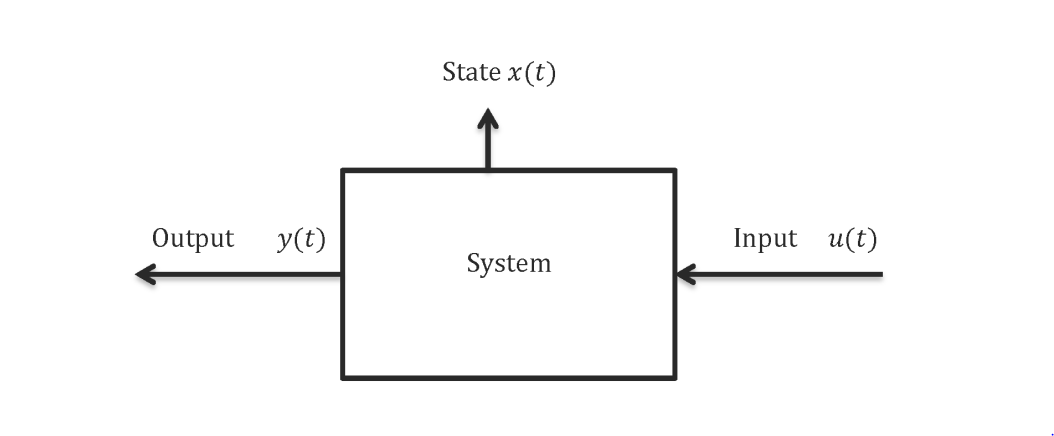
\includegraphics[width=13cm]{Anh1}
  \caption{Sơ đồ khối mô hình không-thời gian liên tục.}
  \label{fig:pic1}
\end{figure}
\begin{example}
Để minh họa rõ hơn việc lập công thức không gian trạng thái, ta xét hệ 2 vật nặng được nối với nhau bởi một lò xo và giảm chấn. Lực $\emph{u}$ tác động vào vật $M_1$, làm thay đổi vị trí $\emph{z}$ của vật $M_2$. Đầu vào của hệ này là lực tác động, đầu ra chính là vị trí của vật $M_2$. Ở đây thứ ta cần quan tâm chính là việc ta có thể điều khiển được vị trí của $M_2$.\\
Áp dụng định luật II Newton, ta có:
\begin{align}
    M_1\ddot{w} &= -b(\dot{w} - \dot{z}) - k(w - z) + u, \\
    M_2\ddot{z} &= b(\dot{w} - \dot{z}) + k(w - z).
\end{align}

\begin{figure}[htp]
\centering
  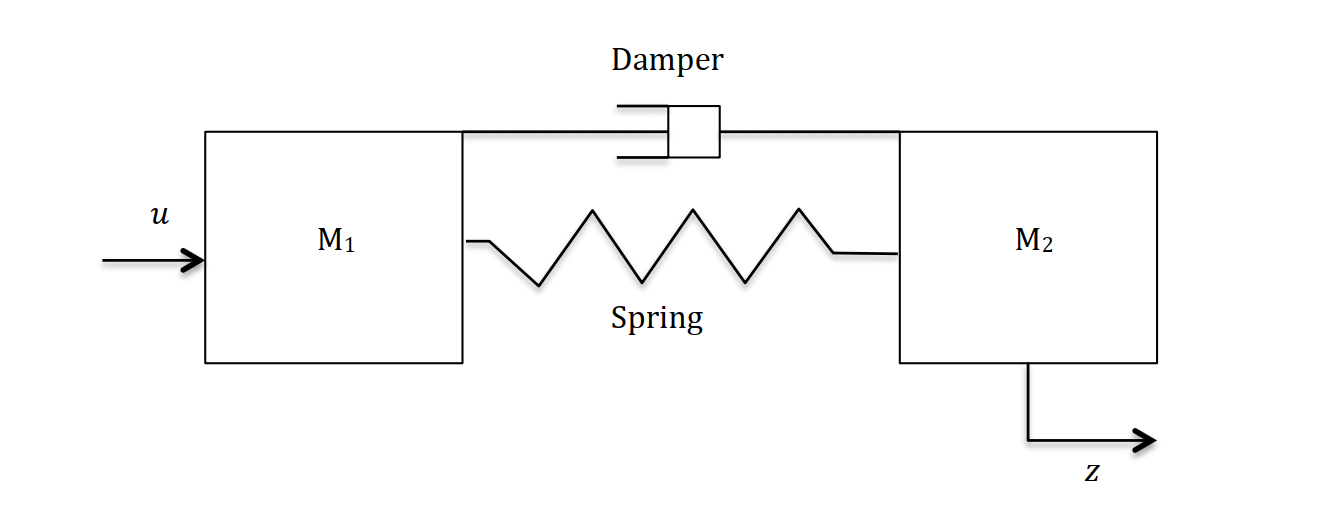
\includegraphics[width=13cm]{Anh2}
  \caption{Hệ vật lò xo giảm chấn.}
  \label{fig:pic2}
\end{figure}

Ở đây, b là hệ số tắt dần, w và z liên tục là sự dịch chuyển  $M_1$ và $M_2$, k là độ cứng của lò xo. Ta đưa hệ đạo hàm bậc 2 này về bậc 1 bằng cách:\\
Đặt $x_1$ = w, $\dot{x_1}$ = $\dot{w}$ = $x_2$, $x_3$ = z, $\dot{x_3}$ = $\dot{z}$ = $x_4$. Khi đó,
\begin{align}
\dot{x}_2 &= -\frac{b}{m_1}(x_2 - x_4) - \frac{k}{m_1}(x_1 - x_3) + u \label{ct2.1.4},  \\
\dot{x}_4 &= \frac{b}{m_2}(x_2 - x_4) + \frac{k}{m_1}(x_1 - x_3) + u, \\
y &= x_3.\label{ct2.1.6}
\end{align}
Ta viết lại \eqref{ct2.1.4}-\eqref{ct2.1.6} hệ dưới dạng ma trận
\begin{align}
    \begin{bmatrix}
        \dot{x}_1\\ \dot{x}_2\\ \dot{x}_3\\ \dot{x}_4
    \end{bmatrix}
     &= 
    \begin{bmatrix}
     0 & 1 & 0 & 0\\
     -\frac{k}{m_1} & -\frac{b}{m_1} & \frac{k}{m_1} & \frac{b}{m_1}\\
     0 & 0 & 0 & 1\\
     \frac{k}{m_2} & \frac{b}{m_2} & -\frac{k}{m_2} & -\frac{b}{m_2}
     \end{bmatrix}
     \cdot
     \begin{bmatrix}
     x_1 \\ x_2 \\ x_3 \\ x_4
     \end{bmatrix}
     + 
     \begin{bmatrix}
     0 \\ \frac{1}{m_1} \\ 0 \\ 0
     \end{bmatrix}
     \cdot u,\\
     y &= 
     \begin{bmatrix}
     0 & 0 & 1 & 0 
     \end{bmatrix}
     \cdot
     \begin{bmatrix}
     x_1 \\ x_2 \\ x_3 \\ x_4
     \end{bmatrix}.
\end{align}
Ta đưa hệ lò xo-giảm chấn này về dạng \eqref{ct2.1.1}
\bigskip
ta có
\newline
A = $\begin{bmatrix}
     0 & 1 & 0 & 0\\
     -\frac{k}{m_1} & -\frac{b}{m_1} & \frac{k}{m_1} & \frac{b}{m_1}\\
     0 & 0 & 0 & 1\\
     \frac{k}{m_2} & \frac{b}{m_2} & -\frac{k}{m_2} & -\frac{b}{m_2}
     \end{bmatrix}
\quad B = \begin{bmatrix}
     0 \\ \frac{1}{m_1} \\ 0 \\ 0
     \end{bmatrix}
\quad C = \begin{bmatrix}
     0 & 0 & 1 & 0 
     \end{bmatrix}
\quad D = 0.$
\end{example}

\section{Nghiệm không gian trạng thái}
Nếu ta đã biết vector \emph{u}, hệ \eqref{ct2.1.1} có thể giải được. Trước khi đi vào cụ thể, ta cần biết một vài định nghĩa \cite{5}.
\begin{definition}
Cho ma trận A cỡ n $\times$ n, khi đó ta định nghĩa \textbf{hàm mũ ma trận} là \[ e^{At} = \sum_{k = 0}^{\infty} \frac{(At)^k}{k!} .\]
\end{definition}
Hai điều lưu ý về hàm mũ ma trận:\\
1. \emph{$e^{A0} = A^0 = I$}. \\
2. \emph{$\frac{d}{dt}e^{At} = \sum_{k = 0}^{\infty} \frac{d}{dt} \frac{A^k t^k}{k!} = \sum_{k = 1}^{\infty} \frac{A^k t^{k-1}}{(k-1)!} = \sum_{k = 0}^{\infty}A\frac{A^k t^k}{k!} = Ae^{At}$}.\\
Ta biết nghiệm của bài toán giá trị ban đầu
\begin{align}
    \dot{x}(t) = Ax(t),\; x(t_0) = x_0, 
\end{align}
là x(t) = $e^{A(t-t_0)}x_0$.\\
Trở lại với phương trình tổng quát với u cho trước,
\begin{align}
    \dot{x}(t) &= Ax(t) + Bu(t), \; x(t_0) = x_0 \label{ct2.2.2} \\ 
    y(t) &= Cx(t) + Du(t). \label{ct2.2.3}
\end{align}
ta sẽ tìm nghiệm qua biến đổi Laplace.
\begin{definition}[Biến đổi Laplace]
Hàm f(x), x $\in$ [0,$\infty$) có biến đổi Laplace là tích phân $\mathcal{L}(f(x))(s)$ = $\hat{f}$(s) = $\displaystyle \int_1^\infty f(x)e^{-sx}dx$ với giá trị s $\in$ $\mathbb{C}$ mà tích phân có nghĩa.
\end{definition}
Hàm Laplace ngược của $\hat{f}$, ký hiệu bởi $\mathcal{L}^{-1} \hat{f}$ = f, là hàm f sao cho biến đổi Laplace của hàm đó chính bằng $\hat{f}$.\\
Để có thể tìm được nghiệm cho hệ phương trình \eqref{ct2.2.2} - \eqref{ct2.2.3}, ta biến đổi Laplace phương trình \eqref{ct2.2.2} và tìm nghiệm $\hat{x}$, cho ta kết quả là
\begin{align}
    \hat{x}(s) = (sI - A)^{-1} x_0 + (sI - A)^{-1} B \hat{u}(s). \label{ct2.2.4}
\end{align}
Áp dụng hàm Laplace ngược \eqref{ct2.2.4} cho ta nghiệm
\begin{align}
    x(t) &= L^{-1}((sI - A)^{-1} x_0) + L^{-1}((sI - A)^{-1} B \hat{u}(t)) \nonumber\\
         &= e^{A(t-t_0)}{x_0} + \displaystyle \int_{t_0}^t e^{A(t-s)}Bu(s)ds. \label{ct2.2.5}
\end{align}
Ta thay phương trình \eqref{ct2.2.5} vào phương trình \eqref{ct2.2.3} ta tìm được $y(t) = Ce^{A(t-t_0)}x_0 + \int_{t_0}^t Ce^{A(t-s)}Bu(s)ds + Du(t).$
\begin{definition}
Ma trận $e^{A(t-t_0)}$ được gọi là \textbf{ma trận chuyển trạng thái}.
\end{definition}
Nếu ta không biết hàm $\emph{u}$, ta có nhiều phương án điều khiển khác nhau để tìm ra hệ điều khiển có thể cho ra đầu ra mong muốn.

\section{Hàm truyền}
Hàm truyền sẽ cho ta thấy mối quan hệ giữa đầu vào và đầu ra của hệ thống và sự ảnh hưởng của nhiễu đối với đầu ra như thế nào.
Để tìm ra hàm chuyển của hệ \eqref{ct2.1.1}
\begin{align}
    \dot{x}(t) &= Ax(t) + Bu(t), \; x(0) = x_0 \label{ct2.3.1} \\ 
    y(t) &= Cx(t) + Du(t) \nonumber
\end{align}
ta sử dụng biến đổi Laplace như \eqref{ct2.2.4} để thu được nghiệm
\begin{align}
    \hat{x}(s) &= (sI - A)^{-1} x_0 + (sI - A)^{-1} B \hat{u}(s), \label{ct2.3.2}\\
    \hat{y}(s) &= C\hat{x}(s) + D\hat{u}(s). \label{ct2.3.3}
\end{align}
Trừ vế theo vế phương trình \eqref{ct2.3.2} cho phương trình \eqref{ct2.3.3} và đặt G(s) = $\frac{\hat{y}(s)}{\hat{u}(s)}$. Phương trình \eqref{ct2.3.3} trở thành 
\begin{align}
    \hat{y}(s) = G(s)\hat{u}(s), \nonumber
\end{align}
hay 
\begin{align}
    G(s) = \frac{\hat{y}(s)}{\hat{u}(s)}.
\end{align}
Hàm G(s) phản ánh tỷ số giữa đầu ra hệ thống $\hat{y}$(s) và đầu vào hệ thống $\hat{u}(s)$ và được gọi là hàm truyền ma trận hoặc đơn giản chỉ là ma trận truyền. Thành phần $G_{ij}$ trong ma trận biểu diễn hàm truyền từ đầu vào thứ j sang đầu ra thứ i. Hàm truyền này đại diện cho các thuộc tính của hệ thống và không đại diện cho độ lớn hoặc tính chất của các đầu vào. Nó cũng không phục vụ cho việc cung cấp bất kỳ thông tin nào về cấu trúc của hệ thống.\\
Một ưu điểm chính của việc sử dụng hàm truyền là chúng cho phép ta làm việc với một hệ thống phức tạp trong miền thời gian và biểu diễn nó như một hàm của một biến trong miền tần số. Thật không may, cách tiếp cận này chỉ hoạt động đối với các hệ thống đơn đầu ra - đơn đầu vào (SISO). Điều này có nghĩa là, đối với nhiều hệ thống đa đầu vào - đa đầu ra, thì sẽ có nhiều hàm truyền được sử dụng để biểu diễn mỗi quan hệ đầu vào - đầu ra. Cần lưu ý rằng, nhiều hệ thống có thể chia sẻ cùng một hàm truyền, không liên quan đến độ lớn của hệ thống hoặc tính chất của đầu vào.
\begin{definition}
Các điểm p mà tại đó hàm truyền G(p) = $\infty$ được gọi là các cực của hệ.
\end{definition}
Nếu G($\infty$) là một ma trận hằng thì hàm truyền được gọi là \textbf{chính} và nếu G($\infty$) = 0, hàm truyền được gọi là \textbf{chính ngặt}.
Chúng ta hãy sử dụng hệ thống giảm chấn khối lượng lò xo từ Ví dụ \eqref{ct2.1.1} để minh họa cách tìm hàm truyền của một hệ đã cho được mô tả bằng biểu diễn không gian trạng thái.
\begin{example}
Từ Ví dụ \eqref{ct2.1.1} ta có
\begin{math}
A = \begin{bmatrix}
     0 & 1 & 0 & 0\\
     -\frac{k}{m_1} & -\frac{b}{m_1} & \frac{k}{m_1} & \frac{b}{m_1}\\
     0 & 0 & 0 & 1\\
     \frac{k}{m_2} & \frac{b}{m_2} & -\frac{k}{m_2} & -\frac{b}{m_2}
     \end{bmatrix},
\quad B = \begin{bmatrix}
     0 \\ \frac{1}{m_1} \\ 0 \\ 0
     \end{bmatrix},\\
     C = \begin{bmatrix}
     0 & 0 & 1 & 0 
     \end{bmatrix},
\quad D = 0.
\\
\\
\\
Suy \; ra \\
G(s) = C(sI - A)^{-1}B + D = \begin{bmatrix}
0 & 0 & 1 & 0
\end{bmatrix}
\begin{pmatrix}
\begin{bmatrix}
s & 0 & 0 & 0 \\
0 & s & 0 & 0 \\
0 & 0 & s & 0 \\
0 & 0 & 0 & s.
\end{bmatrix}
- 
\begin{bmatrix}
0 & 1 & 0 & 0\\
-4 & -2 & 4 & 2\\
0 & 0 & 0 & 1\\
4 & 2 & -4 & -2
\end{bmatrix}
\end{pmatrix}^{-1}
\begin{bmatrix}
0\\
1\\
0\\
0
\end{bmatrix}.
\end{math}
\end{example}
Giản ước đi ta tìm ra 
\begin{align}
    G(s) = \frac{s + 2}{s^4 + 3s^3 + 6s^2}.\nonumber
\end{align}
\begin{definition}
Trong không gian thời gian - trạng thái biểu diễn ở \eqref{ct2.3.1}, ma trận
\begin{align}
    G(iw) = C(iwI - A)^{-1}B + D
\end{align}
được gọi là \textbf{ma trận phản hồi tần số}, $\omega \in \mathbb{R}$ chính \textbf{tần số}.
\end{definition}

\section{Tính điều khiển được và tính quan sát được}
Tính điều khiển và tính quan sát được là những khái niệm cơ bản của lý thuyết điều khiển. Để trình bày những khái niệm này, ta tham khảo trong mục \cite{5}
\begin{definition}
Hệ \eqref{ct2.1.1} 
\begin{align*}
    \dot{x}(t) &= Ax(t) + Bu(t),\\
    y(t) &= Cx(t) + Du(t)
\end{align*}
được gọi là có thể điều khiển được nếu hệ thống đạt được bất kì trạng thái bất kì $x_1 = x(t_1)$, trong thời gian hữu hạn $t_1$, từ bất kỳ trạng thái ban đầu x(0) bằng cách chọn điều khiển u(t), $0 \leq t \leq t_1$ phù hợp.
\end{definition}
Tính điều khiển của hệ thống \eqref{ct2.1.1}, được gọi là tính điều khiển của cặp (A, B). Định lý sau cung cấp các điều kiện có thể kiểm chứng được về việc một hệ thống có thể điều khiển được hay không.
\begin{theorem}\label{dly2.4.1}
Cho A  $\in \mathbb{R}^{n\times n}$  và  B  $\in \mathbb{R}^{n\times m}(m \leq n).$ Các điều sau đây là tương đương:
 \renewcommand{\theenumiii}{\roman{enumii}}
 \begin{enumerate}
    \item Hệ \eqref{ct2.1.1} có thể điều khiển được.
    \item Ma trận điều khiển $n \times nm$ là $C_M$ = $[B, AB, A^2B,...,A^{n-1}B]$ có đủ hạng dòng.
    \item Ma trận
    \begin{align*}
        W_C = \int_{0}^{t_1}e^{At}BB^{T}e^{A^{T}t}dt
    \end{align*}
không suy biến với bất kỳ $t_1$ > 0.
    \item Nếu ($\lambda$, x) là một cặp giá trị riêng và vector riêng tương ứng của $A^{T}$, thì $x^{T}B \ne$ 0.
    \item Rank(A - $\lambda$ I, B) = n với mọi giá trị riêng $\lambda$ của A.
    \item Các giá trị riêng của A - BK có thể được phân bố tùy ý bằng một lựa chọn thích hợp của K.
 \end{enumerate}
\end{theorem}
\newpage
\begin{definition}
Hệ thời gian liên tục \eqref{ct2.1.1} gọi là $\textbf{quan sát được}$ nếu tồn tại $t_1$> 0 sao cho trạng thái ban đầu x($t_0$) xác định duy nhất nếu biết u(t) và y(t) với mọi $0 \leq t \leq  t_1 $. 
\end{definition}
Tính quan sát được của hệ thống \eqref{ct2.1.1} được gọi là tính quan sát được của cặp (A, C).Tính đối ngẫu có nghĩa là cặp (A, C) có thể quan sát được nếu cặp ($A^{T}, C^{T}$) có thể điều khiển được. Do tính hai mặt của khả năng quan sát và khả năng điều khiển, khả năng quan sát có các đặc điểm tương tự như tính điều khiển được trong Định lý 2.4.1.
\begin{theorem}
Những điều sau đây là tương đương:
\renewcommand{\theenumiii}{\roman{enumii}}
\begin{enumerate}
    \item Hệ \eqref{ct2.1.1} có thể quan sát được.
    \item Ma trận của khả năng quan sát $O_M$ = $[C CA ... CA^{n-1} ]^{T}$ có hạng đủ.
    \item Ma trận
    \begin{align*}
        W_O = \int_{0}^{t_0}e^{A^{T}t}C^{T}Ce^{At}dt
    \end{align*}
không suy biến với mọi $t_1$ dương.
    \item Ma trận 
    \begin{math}
        \begin{bmatrix}
    \lambda I -A \\
    C
    \end{bmatrix}
    \end{math}
có hạng bằng n với mọi giá trị riêng của A.
    \item Nếu ($\lambda$, y) là 1 cặp giá trị riêng và vector riêng của A, thì $C_y \neq$ 0.
    \item Các giá trị riêng cho A - LC có thể được gán tùy ý bằng một lựa chọn thích hợp của L.
\end{enumerate}
\end{theorem}
Khả năng điều khiển và khả năng quan sát đóng vai trò quan trọng trong sự tồn tại của các nghiệm xác định dương và nửa xác định dương cho phương trình Lyapunov.
\begin{definition}
Ma trận A được gọi là \textbf{ma trận ổn định} nếu mọi giá trị riêng của A có phần thực âm thực sự.
\end{definition}
\begin{definition}
Cho A là một ma trận ổn định, thì 
\begin{align}
    C_G = \int_{0}^{t_1}e^{At}BB^{T}e^{A^{T}t}dt
\end{align}
gọi là \textbf{Grammian điều khiển.}
\end{definition}
\begin{definition}
Cho A là một ma trận ổn định, thì
\begin{align}
    O_G = \int_{0}^{\infty}e^{A^{T}t}C^{T}Ce^{At}dt 
\end{align}
được gọi là \textbf{Grammian quan sát.}
\end{definition}
\begin{theorem}\label{dly2.4.3}
Cho A là một ma trận ổn định. Grammian điều khiển $C_G$ thỏa mãn phương trình Lyapunov
\begin{align}
    AC_G + C_GA^{T} = -BB^{T}
\end{align}
và là đối xứng, xác định dương khi và chỉ khi (A, B) có thể điều khiển được.
\end{theorem}
\begin{theorem}\label{dly2.4.4}
Cho A là 1 ma trận ổn định. Grammian quan sát $O_G$ thỏa mãn phương trình Lyapunov
\begin{align}
    O_GA + A^{T}O_G = -C^{T}C
\end{align}
và là đối xứng, xác định dương khi và chỉ khi (A, B) có thể quan sát được.
\end{theorem}
Sau đây là một ví dụ minh họa tính toán của cả 2 giá trị $C_G$ và $O_G$.
\begin{example}
Trở lại hệ \eqref{ct2.1.1}, với 
\begin{align*}
    A = \begin{bmatrix}
        -4 & -8 & -12\\
        0 & -8 & -4\\
        0 & 0 & 0
    \end{bmatrix}, \; B = \begin{bmatrix}
        1\\
        1\\
        1
    \end{bmatrix}, \;  C = [1 \quad 1 \quad 1], \; D = 0.
\end{align*}
Ma trận A ổn định và sử dụng lệnh \textbf{lyap} trong  MATLAB để giải các phương trình Lyapunov trong Định lý 1.4.5 và 1.4.6, chúng ta tìm được
\begin{align*}
    C_G = \begin{bmatrix}
        0.1458 & 0.0208 & 0.0208\\
        0.0208 & 0.0833 & 0.0833\\
        0.0208 & 0.0833 & 0.0833
    \end{bmatrix} = O_G.
\end{align*}
Ta nhận thấy ma trận này có hai dòng bằng nhau nên định thức ma trận bằng 0, suy ra ma trận suy biến, nên (A, B) không điều khiển được và (C, D) không quan sát được.
\end{example}

\section{Tính ổn định hóa được và khả năng phát hiện được}
Một bộ điều khiển thường được thiết kế để ổn định hóa một hệ thống tuyến tính. Điều này được thực hiện bằng cách chọn một điều khiển $u$ thích hợp sao cho ma trận hệ đóng kín $(A - BK)$ ổn định, trong đó $K$ là ma trận phản hồi mà $u(t) = Kx(t)$. Trong phần này, chúng ta xác định tính ổn định hóa được của một hệ thống và trình bày các đặc điểm của hệ thống có thể được ổn định hóa được thông qua điều khiển phản hồi.\\
Đầu tiên chúng ta chọn hệ chưa điều khiển
\begin{align}\label{ct2.5.1}
    \dot{x}(t) = Ax(t), \quad x(0) = x_0.
\end{align}
\begin{definition}
Trạng thái cân bằng của hệ \eqref{ct2.5.1}, là vectơ $x_e$ thỏa mãn
\begin{align}
    Ax_e = 0.
\end{align}
Nếu ma trận A không suy biến, phương trình trên chỉ có nghiệm tầm thường $x_e$ = 0.
\end{definition}
\begin{definition}
Gọi $x_e$ là trạng thái cân bằng của \eqref{ct2.5.1}, thì $x_e$ được gọi là
\begin{enumerate}
    \item ổn định nếu với mỗi $\epsilon$ > 0 tồn tại $\delta$ > 0  sao cho $\norm{x(t) - x_e}$ < $\epsilon$,  $\forall$ t $\geq$ 0 nếu $\norm{x(t_0) - x_e} < \delta$.
    \item ổn định tiệm cận nếu trạng thái cân bằng ổn định và $\exists \delta > 0$ sao cho $\norm{x(t_0) - x_e} < 0$ dẫn đến $\displaystyle \lim_{x\to\infty} x(t) = x_e$.
\end{enumerate}
\end{definition}
Điều này có nghĩa là mọi nghiệm đúng của hệ nếu bắt đầu đủ gần điểm cân bằng ổn định tiệm cận, thì sẽ tiến gần đến điểm cân bằng khi thời gian tăng. Nên nếu $x_e = 0$ và \emph{A} không suy biến, hệ không ổn định được ở trên ổn định tiệm cận nếu $\emph{x(t)} \to 0 \; khi \; \emph{t} \to \infty.$
Các giá trị riêng của ma trận A trong \eqref{ct2.5.1} đặc trưng cho độ ổn định của hệ thống.
\begin{theorem}
Hệ thống \eqref{ct2.5.1} ổn định tiệm cận khi và chỉ khi mọi giá trị riêng của A có phần thực âm thực sự.
\end{theorem}
Cũng như với tính điều khiển, nghiệm của phương trình Lyapunov cũng đặc trưng cho tính ổn định của \eqref{ct2.5.1}.
\begin{theorem}
Hệ:
\begin{align*}
    \dot{x}(t) = Ax(t)
\end{align*}
ổn định tiệm cận khi và chỉ khi với ma trận M đối xứng dương bất kỳ, thì phương trình sau có nghiệm duy nhất
\begin{align*}
    XA + A^{T}X = -M.
\end{align*}
\end{theorem}
Xét hệ tuyến tính \eqref{ct2.1.1},
\begin{align*}
    \dot{x}(t) &= Ax(t) + Bu(t),\\
    y(t) &= Cx(t) + Du(t).
\end{align*}
Ta xét việc tìm nghiệm điều khiển \emph{u} để đưa hệ sang một trạng thái mong muốn. Điều đó có nghĩa là tìm 1 \textbf{ma trận phản hồi} $K$ sao cho $A - BK$ ổn định. Không phải mọi hệ có thể đưa về một trạng thái nhất định, nên điều quan trọng nhất của phần này là tìm ra điều kiện cần và đủ sao cho tồn tại một ma trận phản hồi ổn định.\\
Hơn nữa giả sử ta có thể tìm được mọi thông tin của trạng thái \emph{x(t)} ở mọi thời gian \emph{t} bất kỳ. Sử dụng điều khiển tuyến tính, ta suy ra 
\begin{align}
    u(t) = -Kx(t).
\end{align}
Trừ vế theo vế phương trình \emph{u(t) = -Kx(t)} cho phương trình \eqref{ct2.1.1} ta được \textbf{hệ kín}:
\begin{align}\label{ct2.5.4}
    \dot{x}(t) &= (A - BK)x(t),\\
    y(t) &= (C - DK)x(t).
\end{align}
Ta nhắc lại hệ không điều khiển được \eqref{ct2.5.1}
 ổn định khi ma trận A ổn định. Vậy nên việc ổn định hóa hệ \eqref{ct2.5.4} quy về việc tìm ma trận  $K$ sao cho $(A - BK)$ là ổn định. Nếu tồn tại một ma trận $K$, thì $K$ được gọi là \textbf{ma trận phản hồi} và ổn định hóa được, cặp ma trận (A, B) được gọi là \textbf{cặp ma trận ổn định hóa được}.\\
 Những định lý sau đây cho ta điều kiện cần và đủ để đánh giá việc có thể ổn định được ma trận cho 1 hệ đang xét.\\
 \begin{theorem}
  Những khẳng định sau là tương đương:
 \begin{enumerate}
     \item Cặp ma trận (A, B) là ổn định hóa được.
     \item Rank(A - $\lambda I$, B) = n, với mọi Re($\lambda$) $\geq$ 0.
     \item Với mọi $\lambda$ và x $\ne$ 0, nếu $x^{*}$A = $\lambda x^{*}$ và Re($\lambda$) $\geq$ 0 thì $x^{*}B \ne$ 0.
 \end{enumerate}
 \end{theorem}
 \begin{coroll}
 Nếu cặp (A, B) là điều khiển được,  thì nó cũng ổn định hóa được.
 \end{coroll}
 Lưu ý khả năng điều khiển suy ra khả năng ổn định chỉ là chiều suy ra mà không suy ngược lại.\\
 Cũng như khả năng quan sát được đối ngẫu với khả năng điều khiển được, khả năng ổn định được của hệ thống cũng đối ngẫu với khả năng phát hiện được.\\
 \begin{definition}
 Hệ được gọi là \textbf{phát hiện được} nếu tồn tại ma trận L sao cho với cặp ma trận (A, C) thì A - LC là ổn định.
 \end{definition}
\begin{theorem}
Các điều sau đây là tương đương:
\begin{enumerate}
    \item Cặp ma trận (A, C) là phát hiện được.
    \item Ma trận 
    $\begin{bmatrix}
        \lambda I - A \\
        C.
    \end{bmatrix}$
    có hạng đầy đủ, với mọi $Re(\lambda) \geq$ 0.
    \item Với mọi $\lambda$ và x $\ne$ 0 sao cho Ax = $\lambda$x và Re($\lambda) \geq$ 0, thì Cx $\ne$ 0.
    \item Cặp ma trận ($A^{T}$, $C^{T}$) là ổn định hóa được.
\end{enumerate}
\end{theorem}
Có thể thấy rằng một hệ thống có thể điều khiển được thì các giá trị riêng của hệ điều khiển đóng kín có thể được gán tùy ý (bài toán gán giá trị riêng). Vấn đề với việc chỉ định các giá trị riêng tùy ý đó là không có phương pháp luận để tìm một bộ điều khiển tối ưu sao cho các đặc điểm thiết kế hệ thống có thể đáp ứng một cách hiệu quả nhất có thể.\\
Điều này dẫn đến nhiều phương pháp điều khiển tối ưu ví dụ như điều khiển tối ưu tuyến tính bậc hai. Phương pháp này tối thiểu hóa hàm phạt bậc 2 đã được xác định trước. Tuy nhiên, lưu ý \cite{7} cho ta sự phát triển song song của điều khiển \hinf và điều khiển \emph{$H_2$} tối ưu hay còn được gọi là điều khiển dạng toàn phương tuyến tính Gauss.

\section{Chuẩn \hinf}
Trước tiên, hãy lưu ý rằng hàm truyền của một hệ thống ổn định bất kỳ được mô hình hóa bởi phương trình vi phân tuyến tính hệ số hằng là hàm hữu tỉ và có các cực nằm hoàn toàn trong nửa mặt phẳng bên trái và là giải tích trong nửa mặt phẳng bên phải. Một không gian của các hàm như vậy được gọi là không gian Hardy, ký hiệu là \hinf. Đối với hệ đa biến bất kỳ, hàm truyền G(i$\omega$) là một ma trận. Các giá trị kỳ dị của ma trận A, $\sigma_j$(A) được định nghĩa là
\begin{align*}
    \sigma_j(A) = \sqrt{\lambda_j(AA^{T})},
\end{align*}
trong đó $\lambda_j$(E) là giá trị riêng thứ j của ma trận E.
\newline
\newline
Chuẩn Euclid của ma trận là:
\begin{align*}
    \norm{A} = \displaystyle \max_{i}\sigma_i(A).
\end{align*}
Suy ra
\begin{align*}
    \norm{G(i\omega)} = \displaystyle \max_{i}\sigma_i(G(i\omega)) = \sigma_{max}(G(i\omega)).
\end{align*}
\begin{definition}
Chuẩn \hinf của hàm truyền G(s) được định nghĩa là
\begin{align}
    \norm{G}_{\infty} = \sup_{\omega \in \mathbb{R}}\sigma_{max}(G(i\omega)).
\end{align}
\end{definition}
\smallskip
Chuẩn này cung cấp một cách khác để phân tích tính ổn định của hệ thống, cụ thể là nếu G(s) $\in$ \hinf thì hệ thống ổn định. Như được mô tả trong \cite{15} cho trường hợp khi G là hữu tỉ, G $\in$ \hinf khi và chỉ khi G không có cực trong nửa mặt phẳng đóng bên phải.
\newpage